

\subsection [Xylene degradation (1D)]{1D reactive transport: Xylene degradation with multiple monod kinetics, exchange kinetics and biomass growth}
\label{l_s_benchmark_1d_xylene_deg}

This benchmark describes the reactive transport of xylene in a homogeneous aquifer. The main purpose is to document the ongoing reactions, which are xylene degradation under aerobic, sulfate reducing and iron reducing conditions, considering growth of the respective biomasses. Also included is the rate limited exchange of iron goethite into bioavailable iron. The aquifer is represented by a one-dimensional model of 50 m length in the x-direction and 1 m in the y-and z directions, respectively. The model is discretized by 100 line elements of constant 0.5 m length in x direction. With an isotropic hydraulic conductivity K of 2.13 $\cdot$10$^{-3}$ m s$^{-1}$, a porosity of 0.24 and a hydraulic gradient I of 1.3$\cdot$10$^{-4}$, the steady state transport velocity va is 0.1 m d$^{-1}$. Longitudinal dispersivity  $\alpha_L$ is set to 0.25 m, the diffusion coefficient $D_a$ is set to 1.0$\cdot$10$^{-9}$ m$^2$ s$^{-1}$. The physical aquifer parameters are summarized in Tab.~\ref{l_tab_benchmark_1d_xylene}. The transport simulation is run for a period of 1000 d with a time step length of 5 d.

The model aquifer has a length of 50 m in the x-direction, 1 m in the y-direction and 1 m in the z direction. The whole domain is discretized into 100 line elements with a constant x and y dimension of 1 m.
The aquifer is assumed to have a homogeneous and isotropic hydraulic conductivity. Using a gradient of 1.23 $\cdot$10$^{-4}$ and a porosity of 0.24 produces a steady state transport velocity of 0.10 m d$^{-1}$.

Xylene degradation is simulated according to the typical redox sequence.


\begin{table}[htbp]
\caption{Parameters used for benchmark HC$\backslash$1d\_xylene\_degradation }
\centering
\begin{tabular}{|l|l|l|}
\hline
parameter & value & unit \\
\hline
porosity $\Phi = n $  & 0.24 &  --  \\			
\hline
matrix volume fraction $VOL_MAT $  & 0.75 &  --  \\			
\hline
biomass volume fraction $VOL_BIO $  & 0.01 &  --  \\			
\hline
hydraulic conductivity $K$ & 2.13$\cdot 10^{-3}$ & ms$^{-1}$ \\
\hline
storage coefficient $S$ & 0.0 & s$^{-1}$ \\
\hline
solid density $\rho_s$ & 2000 &  kg$\cdot m^{-3}$ \\
\hline
density of water $\rho_w$ & 1000 & kg$\cdot m^{-3}$ \\
\hline
viscosity water $\eta$ & 0.001 & Pa$\cdot s$ \\
\hline
longitudinal dispersivity $\alpha_l$ & 0.25 & m \\
\hline
component diffusion coefficient $D$ & 1.0$\cdot 10^{-9}$ & m$^2$s$^{-1}$ \\
\hline
\end{tabular}
\label{l_tab_benchmark_1d_xylene}
\end{table}

\subsubsection*{Evaluation method}

Model results are compared an older version of GeoSys/RockFlow.

\subsubsection*{Results}

Results of the simulation are shown in Fig.~\ref{profiles_xylene_degradation} for xylene, the electron acceptors oxygen and sulfate, as well as for the biomass of the aerobic microorganisms, the sulfate reducers and the iron reducers simulation time steps of 100 days.
For simulation time t $<$ 500~d, one can see the advancing xylene front, a reduction of xylene concentrations is only visible for later times, when xylene concentrations reduce to about 90\% of the inflow concentration. Also shown is the increasing consumption of oxygen with time, accompanied by the growth of the aerobic reducers at the inflow (left) end of the model area. After approximately 800~d, oxygen concentrations in the inflowing groundwater are reduced to almost zero within the first 20~m of the aquifer. Sulfate reducers initially decay from their initial amount, as growth is inhibited throughout the column by the still high concentrations of oxygen. Once oxygen is used up, however, sulfate reducers start to grow downstream of the oxygen reducers and sulfate concentrations in the groundwater reduce accordingly. The iron reducers decay from their initial values and start to grow only for late times t $>$ 80~d and x $>$ 30~m, as xylene degradation from iron reduction is inhibited by both, oxygen as well as sulfate, which is still present in concentrations larger than the inhibition concentration for iron reducers. Accordingly, the spatial distribution of bioavailable iron is still almost uniform throughout the aquifer.
%Figure 2 shows the slow temporal decrease of goethite concentrations and the corresponding increase in bioavailable iron concentrations resulting from the slow transfer kinetics.


\begin{figure}[htbp]
\centering
\includegraphics[width=0.9\textwidth]{C/figures/profiles_xylene_degradation.eps}
\caption{Profiles of oxygen, sulfate and xylene (top row, from left) and  aerobic reducers, sulfate reducers and iron reducers at different times during the 1000 d simulation period.}
\label{profiles_xylene_degradation}
\end{figure}


\begin{table}[htbp]
\centering
\begin{tabular}{|l|l|l|}
\hline
Benchmark & Type & Path \\
\hline
\texttt{1d\_xylene\_degradation}& HC &  benchmarks$\backslash$C$\backslash$1d\_xylene\_degradation  \\			
\hline
\end{tabular}
\end{table}




\subsection[Competition of TCE- and cis-DCE-degradation for zero valent iron surface (1D)]{1D reactive transport: Competition of TCE- and cis-DCE-degradation for the zero valent iron surface}
\label{l_s_benchmark_1d_TCEonIon}

This example simulation demonstrates the use of GeoSys/RockFlow for simulation of multi-species kinetic reactions. The reaction system was set up by D. Schäfer and published in Schäfer et al. (2003) (Schäfer, D., R. Köber and A. Dahmke (2003): Competing TCE- and cis-DCE-degradation kinetics by zero-valent iron - experimental results and numerical simulation. Journal of Contaminant Hydrology, 65(3-4): 183-202). Further, it was used for model verification of the newly implemented and developed kinetic reaction module in GeoSys/RockFlow. The example considers flow in a one-dimensional column of 1 m length, resembling the thickness of a reactive iron barrier perpendicular to the flow direction. It involves 19 species and and 16 different geochemical reactions, both first-order degradation reactions of adsorbed substances and kinetic sorption reactions of the langmuir-type, considering competition for the available sorption sites.

The model set up consists of a 1d column with saturated ground water flow with a darcy velocity of 5.0$\cdot$ 10$^{-4}$ m d$^{-1}$ from left to right. Geochemical species are added to the inflowing water, and their sorption and degradation behavior is modeled. For a complete description of input parameters see the paper by Schfer et al. (2003). Every degradation reaction follows a Langmuir-Hinshelwood-Hougen-Watson kinetics with a limited number of sites for the adsorption and desorption of chlorinated hydrocarbons on the reactive iron surface. Since all the reactive substances involved have to adsorb onto the reactive iron surface in order to be degraded, a competition for the surface sites occurs. This competition has been investigated in column studies and the observed concentration profiles were simulated with the numerical model TBC (Schfer et al., 2003).



\subsubsection*{Evaluation method}

Model results are compared an older version of GeoSys/RockFlow, which was compared to the original TBC simulations.

\subsubsection*{Results}

Results of the simulation are shown in Fig.~\ref{profiles_TCEonIon}, where profiles of the dissolved species are shown. TCE and cis-DCE are added to the inflowing water. They compete for the sorption sites, and when sorbed degrade according to a first order degradation reaction. The retardation of the reactive species compared to the conservative tracer \texttt{mobile} is clearly visible. Also, just downstream of the concentration decrease of TCE or cis-DCE, the degradation products ethane and C4-containing molecules increase. These species are again mobile and are transported with the water, so an instationary behaviour is observed in Fig.~\ref{profiles_TCEonIon}.

\begin{figure}[htbp]
\centering
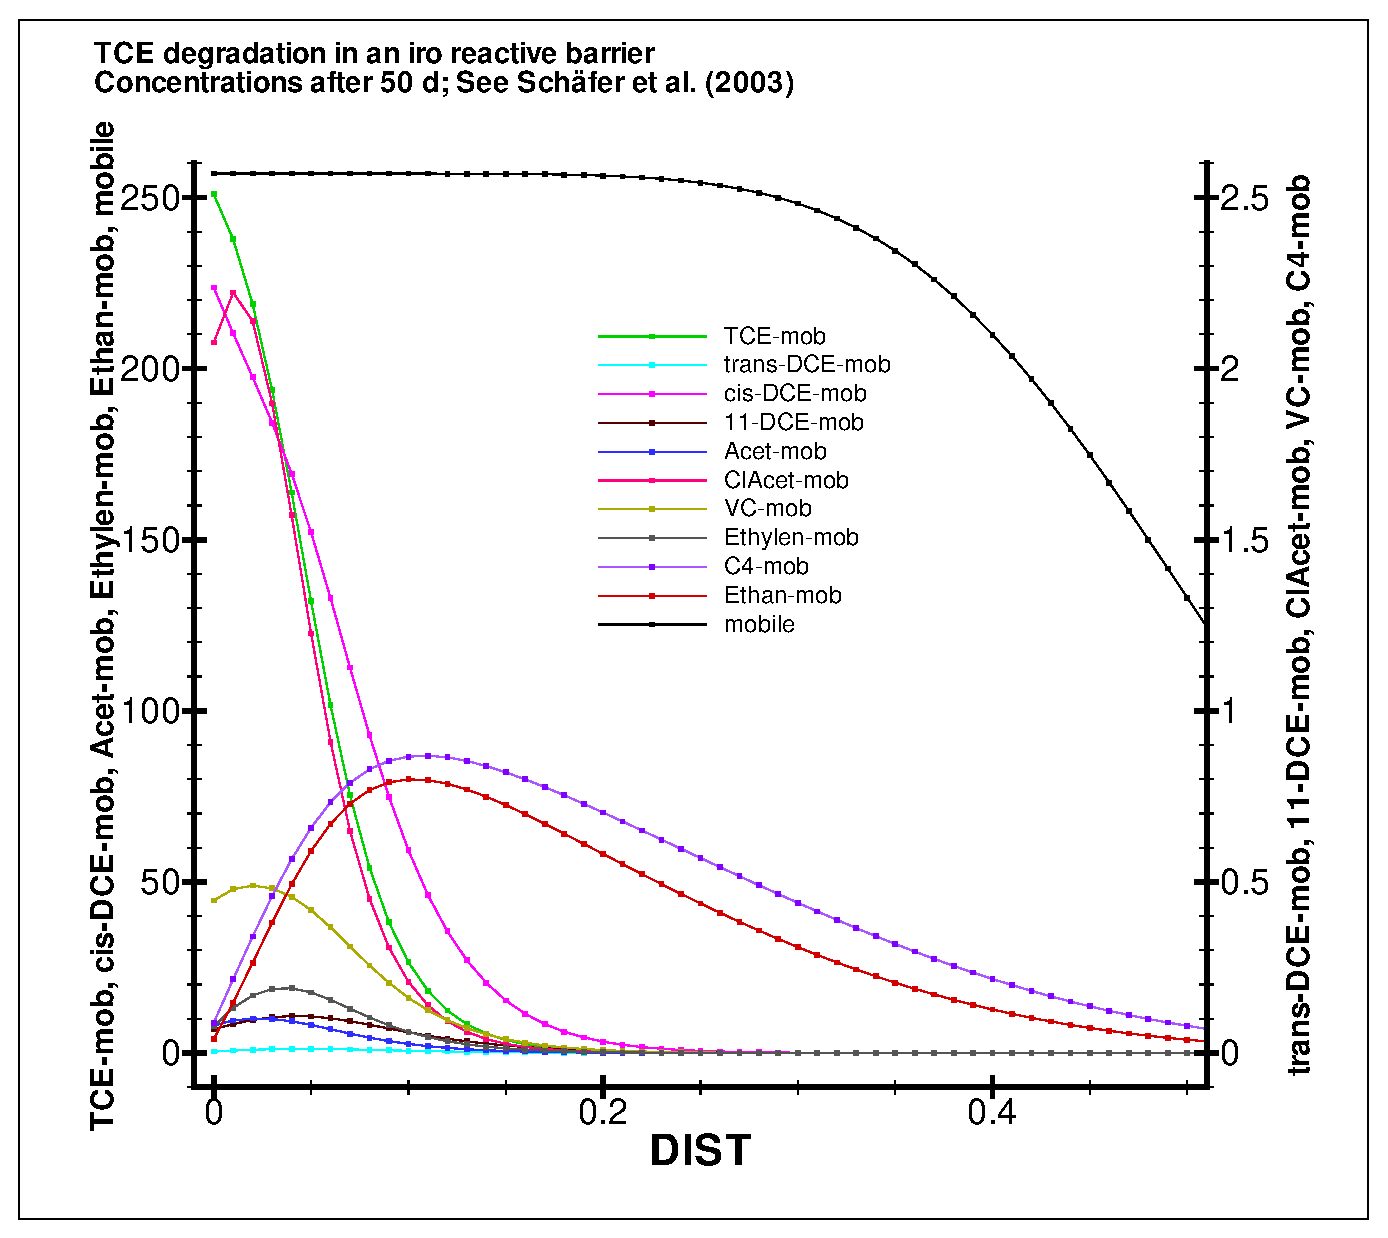
\includegraphics[width=0.9\textwidth]{C/figures/1d_TCEonIon.eps}
\caption{Concentration profiles of TCE, trans-DCE, cis-DCE, 1,1-DCE, Acetylene, chloroacetylene, C4, VC, ethene and ethane as well as the concervative tracer mobile after 50 d simulation time.}
\label{profiles_TCEonIon}
\end{figure}


\begin{table}[htbp]
\centering
\begin{tabular}{|l|l|l|}
\hline
Benchmark & Type & Path \\
\hline
\texttt{1d\_TCEonIon}& HC &  benchmarks$\backslash$C$\backslash$1d\_TCEonIon  \\			
\hline
\end{tabular}
\end{table}



